\section{Logistic Functions}
\label{sec:logistic}

The (fictional) town of Sigmoidville has 5000 people. You and some friends design an app for residents of the town. Table \ref{tab:1-7-app} shows the number of downloads of the app over a span of 90 days.

\begin{table}[!ht]

	\centering
  \begin{tabular}{lrrrrrrrrrr}
    \toprule
    {\bf Day} ($t$)       & 0 & 10 & 20  & 30 & 40 & 50 & 60 & 70 & 80 & 90 \\
    \midrule
    {\bf Downloads} ($D$) & 16 & 52 & 166 & 491 & 1201 & 2127 & 2771 & 3049 & 3144 & 3174   \\
    \bottomrule
\end{tabular}
\caption{Total downloads, $D$, of the Sigmoidville app after $t$ days.}
\label{tab:1-7-app}
\end{table}

You notice that the download rate is slow, then rapid, then slow again. A plot of the data shows that this is indeed the case.

\begin{figure}[!ht]
	\centering
	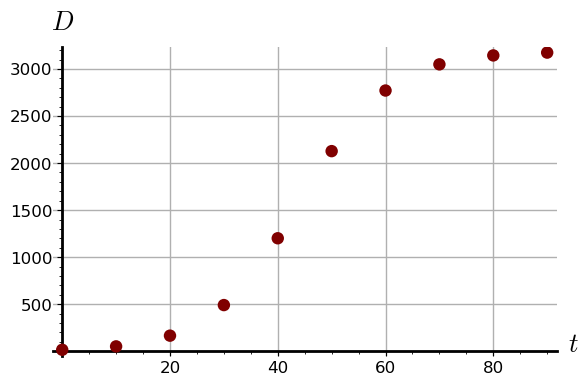
\includegraphics[width = 0.6\textwidth]{img/chap1/sec1-7/1-7-app.png}
	\caption{Total downloads, $D$, of the Sigmoidville app after $t$ days.}
    \label{fig:1-7-app}
	\end{figure}


Why does this make sense? At first, only a few of you know about the app. As you tell others about the app, more will download it and they may tell others about the app as well, so download rates accelerate. However, there are only 5000 people in town and you don't expect anyone outside the town to download it, so eventually the market will be {\bf saturated}. Also, not everyone in town would want the app, so you may not get 5000 total downloads.

This situation is an example of {\bf bounded exponential growth}. In general, a curve called a {\bf logistic curve} models {\bf bounded exponential growth or decay}:  

\begin{definition}[Logistic Function]
  A {\bf logistic function}\index{Function!logistic} is a function of the form
  $$f(x) = \dfrac{L}{1+ae^{-bx}} \enspace .$$
    \begin{itemize}    
    \item If $b>0$, then $f(x)$ increases to the {\bf limiting value}\index{Limit} $L$.
    \item If $b<0$, then $f(x)$ decreases to 0.
    \end{itemize}
\end{definition}

Logistic models apply when there is a limit to the growth of some phenomenon. Examples of logistic models include the following.
    \begin{itemize}
    \item Product sales: an astute inventory manager will note when the total sales of an item have reached an {\bf inflection point} and will stop ordering that item to stock inventory.
    \item Population growth, where limited resources define a {\bf carrying capacity} of the population 
    \item The spread of an infectious disease.
    \end{itemize}

\begin{example} A (slightly simplified) {\bf best fit curve} can be found for the number of downloads of the Sigmoidville app after $t$ days: 
$$D(t) = \frac{3187}{1+201\cdot e^{-0.12t}} \text{ downloads after } t \text{ days.}$$
This tells us that we can expect a total of 3187 app downloads, so you have effectively reached the point of market saturation after 90 days and you can only expect a dozen or so more downloads.

\begin{figure}[!ht]
	\centering
	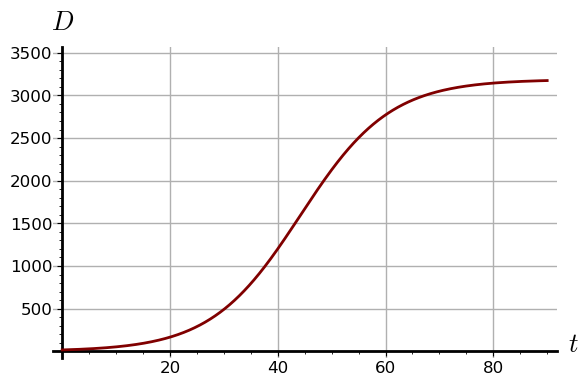
\includegraphics[width = 0.6\textwidth]{img/chap1/sec1-7/1-7-app-graph.png}
	\caption{Modeling the total downloads, $D$, of the Sigmoidville app after $t$ days.}
    \label{fig:1-7-app-graph}
	\end{figure}
\end{example}

You can model logistic growth with a group of people. One or two people are secretly, possibly randomly, chosen to be zombies. There are a number of ``rounds'' in which during each round, everyone shakes hands with another person. Zombies will give an extra squeeze or blink their eyes to indicate they are a zombie. If you shake hands with a zombie, you become a zombie yourself. Everyone must remember which round they became a zombie. Plot the cumulative number of zombies in each round. A plot of the data should look logistic, since there will be rapid growth initially, but as the proportion of zombies increases, there will be more occurrences of zombies shaking hands with other zombies, which does not increase the total number of zombies. Eventually, the whole group of people will be zombies.

